%ju 31-Dez-22 19-Bremsen-I.tex
\section{Bremsanlagen}\label{bremsanlagen}

\textbf{Aufgabe einer Betriebsbremsanlage (BBA)}

\begin{enumerate}
\item
  Fahrzeug im Stillstand halten
\item
  Fahrzeuggeschwindigkeit verringern
\item
  Fahrzeug anhalten
\item
  Fahrzeuggeschwindigkeit im Gefälle halten
\end{enumerate}

\textbf{Aufgabe einer Hilfsbremsanlage (HBA)}

\begin{enumerate}
\item
  Bei Ausfall der Betriebsbremsanlage deren Aufgabe ggf. mit
  verminderter Wirkung übernehmen.
\end{enumerate}

\textbf{Aufgabe einer Feststellbremsanlage (FBA)}

\begin{enumerate}
\item
  Fahrzeug gegen wegrollen sichern
\end{enumerate}

\textbf{Aufgabe einer Dauerbremsanlage (DBA, Retarter)}

\begin{enumerate}
\item
  Fahrzeuggeschwindigkeit im Gefälle halten und verringern
\end{enumerate}

\section{Bremsvorgang}\label{bremsvorgang}

doppelte Geschwindigkeit $\to$ 4-facher Bremsweg

Bremsweg
$\boxed{s = \frac{v \cdot t}{2}} \quad \boxed{1~m/s = 3,6~km/h}$

$s_{40~km/h} = \frac{11~m/s \cdot 2,73~s}{2} = 15~m$

$s_{80~km/h} = \frac{22~m/s \cdot 5,5~s}{2} = 60~m$

Doppelte Masse $\to$ doppelte Bremsarbeit

Bremsarbeit
$\boxed{W_B = \frac{m \cdot v^2_\text{konst}}{2000}} \text{ in kJ}$

$W_{B_{1000~kg}} = \frac{1000~kg \cdot \sim 22^2~m/s^2}{2000} = 242~kJ$

$W_{B_{2000~kg}} = \frac{2000~kg \cdot \sim 22^2~m/s^2}{2000} = 484~kJ$

\newpage

\textbf{Nenne Einflussgrößen für den Bremsweg}

\begin{enumerate}
\item
  Fahrgeschwindigkeit (Faktor 2, doppelte Geschwindigkeit $\to$
  4-facher Bremsweg)
\item
  Fahrzeugmasse (Doppelte Masse $\to$ doppelte Bremsarbeit)
\item
  Fahrbahnzustand (trocken, nass, verreist)
\item
  Reifenzustand (Alter, Fülldruck, Profiltiefe)
\item
  Zustand der Bremse (schwergängig, Belag verglast)
\item
  Zustand der Stoßdämpfer
\item
  Bremskraftregelung (ABS)
\end{enumerate}

\textbf{Beispiel Bremskraftleistung eines Lkw}

$\boxed{t = \frac{2 \cdot s}{v_\text{konst}}} \quad \boxed{1~m/s = 3,6~km/h}$

$t_\text{Beschleunigung} = \frac{2 \cdot 660~m}{\sim 22~m/s} = 60~s$

$t_\text{Bremsen} = \frac{2 \cdot 60~m}{\sim 22~m/s} = 5,5~s$

\begin{itemize}
\item
  Beschleunigung 660 m in \textbf{60 s} auf 80 km/h (ca. 22 m/s)
\item
  Negative Beschleunigung (Bremsen) 60 m in \textbf{5,5 s} bis zum
  Stillstand
\end{itemize}

\newpage

\section{Hydraulische Bremse}\label{hydraulische-bremse}

\textbf{Pascalsche Gesetz} der auf eine eingeschlossene Flüssigkeit
ausgeübte Druck überträgt sich in dieser nach allen Richtungen
gleichmäßig.

Die hebelübersetze Pedalkraft wird im Bremskraftverstärker um den Faktor
4 -- 10 verstärkt und wirkt auf die Kolben im Hauptbremszylinder. Die
Bestätigungskraft wird in einen hydraulischen Druck umgewandelt. Diese
liegt bei Vollbremsung im Bereich zwischen 100 -- 160 bar.

\textbf{Zusammenhang Druck, Fläche, Kraft und Weg}

$\boxed{A = \frac{\pi \cdot d^2}{4}} \quad \boxed{F = p_\text{konst} \cdot A} \quad \boxed{W = F \cdot s} \quad \boxed{i = \frac{s_2}{s_1}} \quad \boxed{1~bar = 10~N/cm^2}$

\begin{itemize}
\item
  \textbf{geg:}

  \begin{itemize}
  \item
    $d_1 = 50~mm = 5~cm, d_2 = 71,36~mm = 7,136~cm, p = 10~bar = 100~N/cm^2$
  \end{itemize}
\item
  kleine Fläche und kleine Kraft
  $A_1 = \frac{\pi \cdot 5^2}{4} = 20~cm^2 \quad F_1 = \sim 10~bar \cdot 20~cm^2 = 200~N$
\item
  große Fläche und große Kraft
  $A_2 = \frac{\pi \cdot 7,136^2}{4} = 40~cm^2 \quad F_2 = \sim 10~bar \cdot 40~cm^2 = 400~N$
\end{itemize}

\begin{figure}[!ht]% hier: !ht
\centering
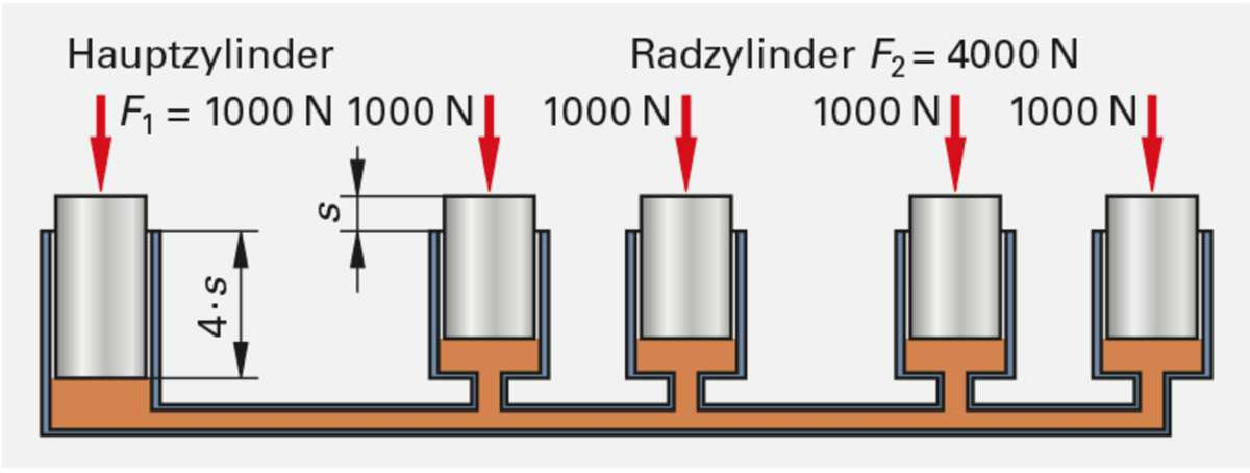
\includegraphics[width=0.5\textwidth]{images/Bremsen/Bremsen-1.pdf}
\caption{hydraulischen Bremse, Quelle: Europa-Verlag}
%\label{fig:}%% anpassen
\end{figure}

\begin{itemize}
\item
  \textbf{geg:}

  \begin{itemize}
  \item
    $p_\text{max} = 180~bar = 1800~N/cm^2, F_\text{Hauptbremszylinder} = 1000~N, F_\text{4x Radzylinder} = 4000~N$,
    $s_\text{Hauptbremszylinder} = 8~mm, s_\text{4x Radzylinder} = 2~mm$
  \end{itemize}
\item
  kleine Kolbenfläche
  $A_\text{Hauptbremszylinder} = \frac{1000~N}{1800~N/cm^2} = 0,55~cm^2$
\item
  große Kolbenfläche
  $A_\text{4x Radzylinder} = \frac{4000~N}{1800~N/cm^2} = 2,22~cm^2$
\item
  übersetzung: 4x Kolbenweg am Hauptbremszylinder
  $i = \frac{2~mm}{8~mm} = 0,25 = 1:4$
\item
  gleiche Arbeit
  $W_\text{Hauptbremszylinder} = 1000~N \cdot 0,008~m = 8~Nm$
\item
  gleiche Arbeit
  $W_\text{4x Radzylinder} = 4000~N \cdot 0,002~m = 8~Nm$
\end{itemize}

\textbf{Nenne Vorteile einer hydraulischen Bremsanlage}

\begin{enumerate}
\item
  Drücke bis 180 bar
\item
  Geringe Flüssigkeitsmengen durch kleine Abmessungen der hydraulischen
  Bremsanlage
\item
  Kleines Lüftspiel
\item
  wartungsarm
\end{enumerate}

\newpage

\section{Bremskraftaufteilung}\label{bremskraftaufteilung}

\textbf{Welche Aufteilung von Bremskreisen gibt es?}

\begin{figure}[!ht]% hier: !ht
\centering
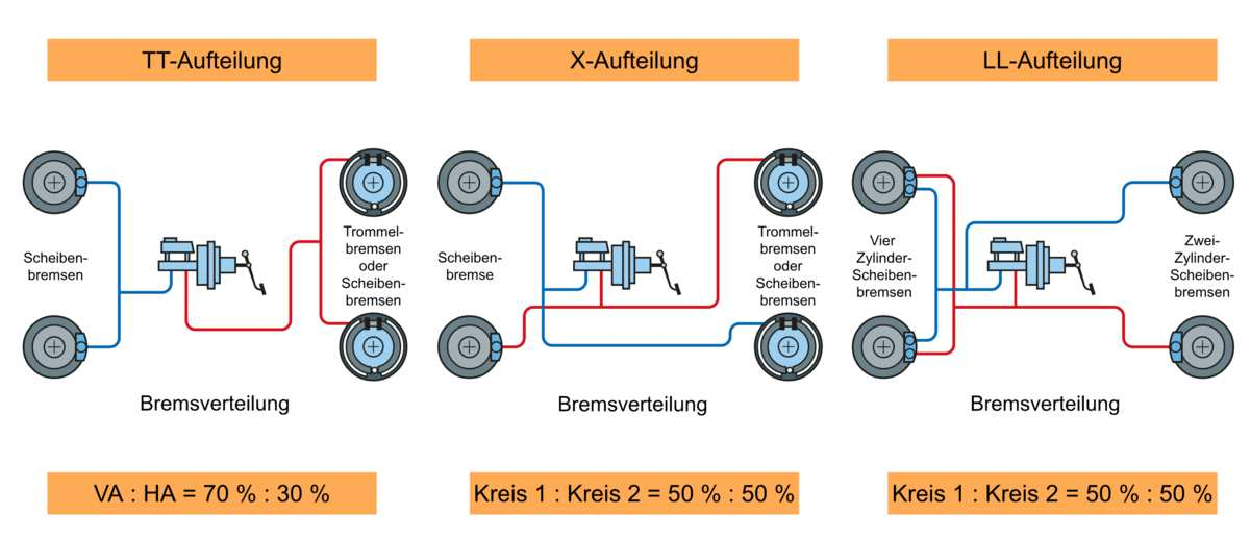
\includegraphics[width=0.5\textwidth]{images/Bremsen/Bremsen-2.pdf}
\caption{Bremskreisaufteilungen, Quelle: Europa-Verlag}
%\label{fig:}%% anpassen
\end{figure}

\begin{enumerate}
\item
  II / TT (Schwarz-weiß) Bremskreis 1 (VA) und Bremskreis 2 (HA)

  \begin{itemize}
  \item
    Bremskraftverteilung VA : HA (70 \% : 30 \%)
  \end{itemize}
\item
  X (Diagonal) Bremskreis 1 (VA links + HA rechts) und Bremskreis 2 (VA
  rechts + HA links)

  \begin{itemize}
  \item
    Bremskraftverteilung Kreis 1 : Kreis 2 (50 \% : 50 \%)
  \end{itemize}
\item
  LL (Dreieck) Bremskreis 1 (VA + HA rechts) und Bremskreis 2 (VA + HA
  links)

  \begin{itemize}
  \item
    Bremskraftverteilung Kreis 1 : Kreis 2 (50 \% : 50 \%)
  \end{itemize}
\end{enumerate}

\textbf{Warum gibt es eine Bremskreisaufteilung?}

Sicheres Abbremsen des Fahrzeugs gewährleisten, bei Ausfall eines
Bremskreises.

\newpage

\section{Hauptbremszylinder}\label{hauptbremszylinder}

\begin{figure}[!ht]% hier: !ht
\centering
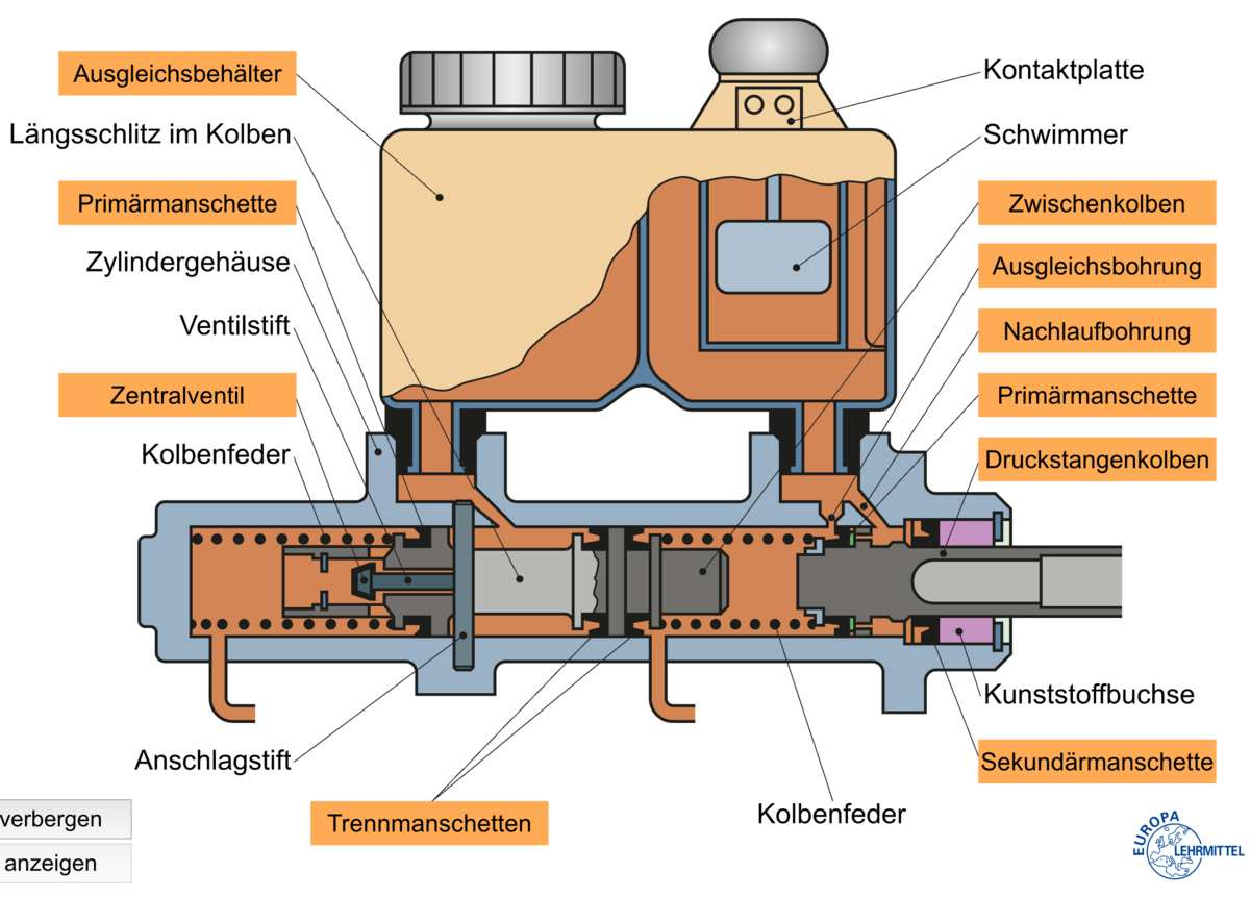
\includegraphics[width=0.5\textwidth]{images/Bremsen/Bremsen-3.pdf}
\caption{Tandem-Hauptbremszylinder, Quelle: Europa-Verlag}
%\label{fig:}%% anpassen
\end{figure}

\textbf{Welche Aufgabe hat der Tandem-Hauptbremszylinder}

\begin{enumerate}
\item
  Umwandeln der Bremskraft in Bremsdruck in der Bremsanlage
\item
  schneller Druckaufbau ermöglichen
\item
  schneller Druckabbau zum Lösen der Bremse
\item
  Absicherung der Bremskreise 1 und 2
\item
  schnelles überwinden der Lüftspiele (Anlegen der Beläge an die
  Scheibe)
\end{enumerate}

\textbf{Primärmanschette} Die Primärmanschette dichtet den Druckraum
beim Bremsvorgang ab, wird beim Schnelllösevorgang als Ventil wirksam
und ermöglicht so das >>Nachsaugen<<.

\textbf{Füllscheibe/Ringscheibe} (Stahl oder Messing) Die Füllscheibe
schützt die Primärmanschette vor Beschädigungen durch die Füllbohrungen
des Kolbens beim Bremsvorgang und wird beim Lösevorgang als Ventil
wirksam.

\textbf{Sekundärmanschette/Ringmanschette} Diese Manschette dichtet den
Ringraum ab. Sie verhindert den Austritt von Flüssigkeit und im
Normalfall auch den Eintritt von Luft

\textbf{Ausgleichsbohrung} ($\varnothing 0,7~mm$) Das
Flüssigkeitsvolumen im Druckraum bei Temperaturschwankungen und beim
Lösevorgang auszugleichen.

\textbf{Nachfüllbohrung} ($\varnothing 3 - 5~mm$) Den Ringraum beim
Lösevorgang auffüllen und einen Lufteintritt in das Bremssystem
verhindern.

\textbf{Zentralventil} verhindert eine Beschädigung der Primärmanschette
des Zwischenkolbenkreises, sobald der dort angeschlossene
Hinterachskreis Blockierneigung aufweist und das ABS dort den
hydraulischen Druck pulsierend regelt.

\textbf{Hochdruckprüfung} 50 -- 100 bar, Prüfdauer 10 Min. (darf max. 10
\% abfallen)

\begin{itemize}
\item
  Undichtigkeit im Bremssystem prüfen
\end{itemize}

\textbf{Niederdruckprüfung} 2 -- 5 bar, Prüfdauer 5 Min. (darf nicht
abfallen)

\begin{itemize}
\item
  Hauptbremszylinder überprüfen

  \begin{itemize}
  \item
    Undichtigkeit am Zentralventil oder an der Primär- oder
    Trennmanschette eines Kolbens
  \end{itemize}
\end{itemize}

\newpage

\section{Trommelbremse}\label{trommelbremse}

\textbf{Nenne Eigenschaften einer Trommelbremse}

\begin{enumerate}
\item
  Selbstverstärkung (Nachteil: keine Dosierbarkeit der Bremskraft)
\item
  Schmutz geschützter Aufbau
\item
  Geringer Bremsbelagverschleiß
\item
  schlechte Wärmeabfuhr
\item
  Neigung zum Fading
\item
  FBA ist einfacher zu integrieren
\end{enumerate}

\textbf{Selbstverstärkung}, die auflaufende Bremsbacke zieht in die
Trommel hinein und verstärkt die Bremswirkung.

\textbf{Bremsfading} Nachlassen der Bremswirkung durch
Temperatureinfluss / Überhitzung. (Bemerkung: Gaspolster entstehen.
Reibzahl des Belags nimmt bei hoher Temperatur ab.)

\textbf{Bremsenkennwert C - Selbstverstärkung} ist abhängig von der
Bauart der Bremse

\textbf{Bauarten einer Trommelbremse}

\begin{figure}[!ht]% hier: !ht
\centering
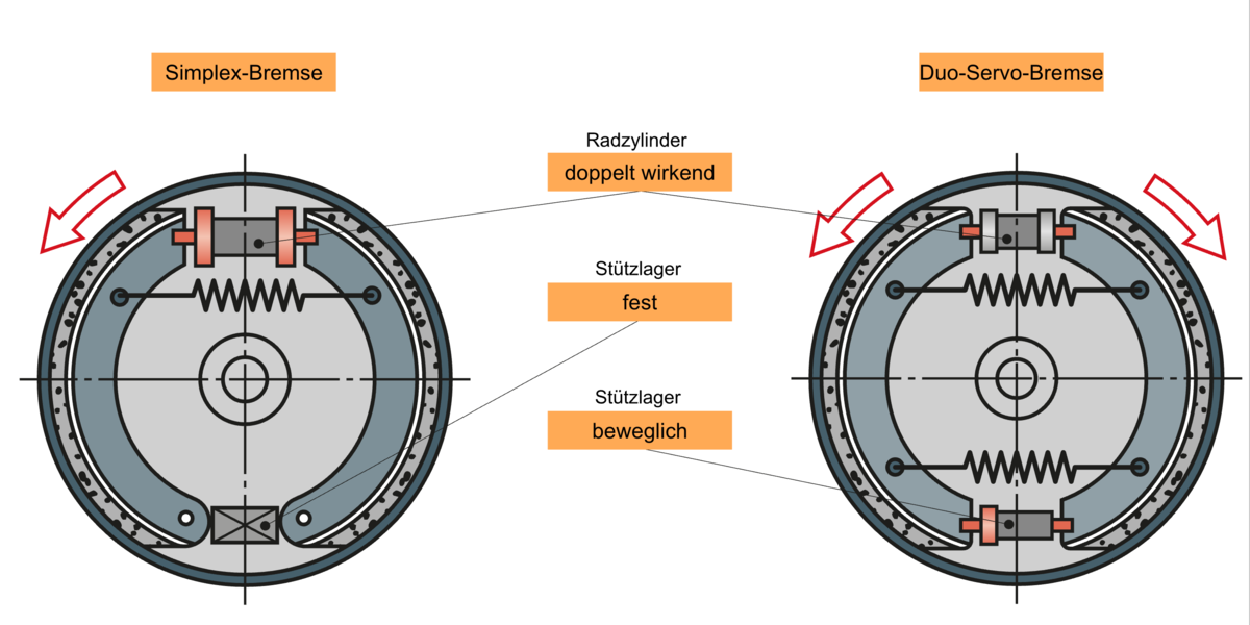
\includegraphics[width=0.5\textwidth]{images/Bremsen/Bremsen-4.pdf}
\caption{Bauarten von Trommelbremsen, Quelle: Europa-Verlag}
%\label{fig:}%% anpassen
\end{figure}

\begin{enumerate}
\item
  \textbf{Duo-Servo-Bremse}

  \begin{itemize}
  \item
    Die untere Abstützung der Bremsbacken nach beiden Seiten beweglich.
  \item
    Es laufen beide Backen bei Vorwärts und Rückwärtsfahrt
    selbstverstärkend auf.
  \end{itemize}
\item
  \textbf{Simplex-Bremse}

  \begin{itemize}
  \item
    Ein Radzylinder mit seinen zwei Kolben betätigt die Bremsbacken.
  \item
    Die Abstützung der Backen erfolgt unten am festen Stützlager.
  \item
    Es gibt bei einer Bremsung in beiden Fahrtrichtungen immer eine
    auflaufende und eine ablaufende Bremsbacke.
  \end{itemize}
\item
  \textbf{Duplex-Bremsen}

  \begin{itemize}
  \item
    Es gibt zwei einseitig wirkende Radzylinder, je Bremsbacke einer.
  \item
    Bei Vorwärtsfahrt wirken beide Bremsbacken auflaufend, also beide
    selbstverstärkend.
  \item
    Bei Rückwärtsfahrt wirken beide Bremsbacken ablaufend, somit ergibt
    sich dann nur eine relativ geringe Bremswirkung.
  \end{itemize}
\end{enumerate}

\textbf{Radbremszylinder} hydraulische Druck wirkt auf einen Kolben und
erzeugt die Spannkraft. Abdichtung durch Nutringmanschette.

\newpage

\section{Scheibenbremse}\label{scheibenbremse}

\textbf{Nenne Eigenschaften einer Schreibenbremse}

\begin{enumerate}
\item
  Verbesserung der Wärmeabfuhr durch innenbelüftete Bremsscheiben
\item
  geringe Neigung zum Fading
\item
  gute Dosierbarkeit der Bremskraft
\item
  höherer Belagverschleiß
\item
  Keine Selbstverstärkung
\item
  gute Kühlung
\item
  Wartung und Belagwechsel einfach
\item
  Selbsttätige Nachstellung des Lüftspiels
\item
  stärkere Erwärmung der Bremsflüssigkeit
\item
  Gefahr der Dampfblasenbildung
\end{enumerate}

\textbf{Bauarten von Scheibenbremsen}

\begin{enumerate}
\item
  \textbf{Festsattel-Scheibenbremse} (mehrere Kolben)
\item
  \textbf{Faustsattel-Scheibenbremse} (ein Kolben)

  \begin{itemize}
  \item
    Geringes Gewicht
  \item
    Kleine Baugröße
  \item
    Gute Wärmeableitung
  \item
    Große Belagflächen
  \item
    Geringer Platzbedarf
  \item
    Geringe Neigung zur Dampfblasenbildung (Bremszylinder ist nur auf
    der Halterseite)
  \item
    Wartungsfreie Gehäuseführung (unempfindlich gegen Schmutz)
  \end{itemize}
\item
  \textbf{Schwimmsattel-Scheibenbremse}
\end{enumerate}

\textbf{Wie erfolgt die Nachstellung bei Scheibenbremsen?
(Kolbenrückstellung)}

\begin{itemize}
\item
  Nach Beendigung des Bremsvorganges und Abbau des Bremsdruckes werden
  die Bremskolben durch das Entspannen des Rechteckringes in ihre
  Ausgangslage gebracht.
\item
  \textbf{Lüftspiel} 0,15 mm.
\item
  Dieser Vorgang kann durch Spreizfedern unterstützt werden.
\end{itemize}

\textbf{Was kann ein Lenkradflattern beim Bremsen verursachen?}

\begin{itemize}
\item
  Radlagerspiel zu groß
\item
  Bremsscheibenschlag zu groß
\end{itemize}

\textbf{Wozu dient eine gelochte oder geschlitzte Bremsscheibe?}

\begin{itemize}
\item
  bei nassen Scheiben schnelle Abfuhr des Wassers
\item
  bessere Kühlung
\item
  bessere Schmutz-, Wasser- und Wärmeabfuhr
\end{itemize}

\textbf{Bremsscheibe}

Die Größe der Bremsscheibe ist ausschlaggebend für das am Rad zur
Verfügung stehende Bremsmoment (ergibt sich aus dem Hebelarm) sowie die
Wärmeabfuhr und Lebensdauer der Scheibe.

Zur besseren Wärmeabfuhr ist sie heutzutage in der Regel innenbelüftet.
Zur besseren Wasser und Schmutzbeseitigung kann sie zudem gelocht oder
geschlitzt sein.

\textbf{Material Kohlefaserverstärkte- oder Keramik-Carbon Bremsscheibe}

\begin{itemize}
\item
  ca. 70 \% leichter
\item
  Hitzebeständigkeit bis zu $1600^\circ\text{C}$ (Vgl. Stahlscheibe
  $800^\circ\text{C}$ Kirschrot)
\item
  nahezu konstanter Reibwert bei Erreichen der Betriebstemperatur
\item
  geringer Verschleiß
\item
  kostenintensiv
\end{itemize}

\textbf{Was bringt es, wenn eine Bremse leichter ist?}

\begin{itemize}
\item
  Weniger \textbf{ungefederte Massen} (alles unterhalb des Stoßdämpfer
  -befestigungspunktes)
\item
  geringere Massenträgheit
\end{itemize}

\textbf{Nenne fünf Anforderungen von Bremsbelägen}

\begin{enumerate}
\item
  Hitzebeständigkeit
\item
  hohe Standzeit
\item
  Wasser und Schmutz unempfindlich
\item
  gleichbleibende hohe Reibungszahl ($\mu$)
\item
  hohe mechanische Festigkeit
\item
  Kein \textbf{Verglasen} (schlechtere Reibungszahl, Scheibe bekommt
  Riefen)
\end{enumerate}

\textbf{Bremsbelag}

\begin{itemize}
\item
  Asbest wurde in Deutschland 1993 verboten und bis 42 \% in Bremsbelag
  enthalten
\item
  mit Prüfzeichen ($E_1$, ECE Genehmigungsnummer) diese belegen, dass
  der Bremsbelag geprüft wurde

  \begin{itemize}
  \item
    gleicher Reibwert wie Original-Beläge des Herstellers
  \item
    Abweichung bis $\pm15 \%$ sind erlaubt
  \item
    Druck- und Scherfestigkeit
  \item
    Asbestfreiheit
  \end{itemize}
\end{itemize}

Eine Prüfnummer mit (E) beginnend, muss am Ersatzteil dauerhaft
identifizierbar vorhanden sein. Die Verpackung der Beläge muss verklebt
oder versiegelt sein, um vorheriges Öffnen klar zu erkennen. Auf der
Verpackung müssen die für den Belag zugelassenen Fahrzeuge gelistet
sein.

\textbf{Arten von Bremskraftverstärkern} (Hilfskraft, Fußkraft des
Fahrers unterstützen)

\begin{enumerate}
\item
  Unterdruck-Bremskraftverstärker

  \begin{itemize}
  \item
    Die geringe \textbf{Druckdifferenz} zwischen Luftdruck 1 bar und
    Saugrohrdruck von etwa 0,2 Bar erfordert große Flächen des
    Arbeitskolbens, um die Druckstangenkraft um den Faktor 4 -- 10 zu
    verstärken.
  \item
    \textbf{Unterdruckerzeugung}

    \begin{itemize}
    \item
      \emph{Dieselmotor:} vom Motor angetriebene Vakuumpumpe
    \item
      \emph{Saug-Ottomotor:} wird dem Ansaugrohr entnommen
    \item
      \emph{Hybridfahrzeug:} Elektrische Vakuumpumpe
    \end{itemize}
  \end{itemize}
\item
  Tandem-Bremskraftverstärker
\item
  Pneumatischer Bremskraftverstärker
\item
  Hydraulischer Bremskraftverstärker
\item
  Elektro-mechanischer Bremskraftverstärker (eBKV, Unterdruck ist nicht
  erforderlich)

  \begin{itemize}
  \item
    Tandem-Hauptbremszylinder mit Vorratsbehälter
  \item
    Elektromotor mit Getriebe und Verstärkungselement
  \item
    Steuergerät
  \item
    Differenzwegsensor
  \end{itemize}
\end{enumerate}

\textbf{Blended Braking} Überlagerung von elektrischem Bremsen
(Rekuperation des Drehstrommotors) + hydraulischem Bremsen = gewünschte
Verzögerung des Fahrers

\textbf{Bremsassistent (BAS)} ab einer bestimmten
Pedalweggeschwindigkeit (Membranwegsensor dient zur Berechnung) wird von
einer Notbremsung ausgegangen, und die Bremsassistentfunktion wird
ausgelöst. Dafür wird im Bremskraftverstärker ein Magnetventil (BAS)
geschaltet, das die Arbeitskammer belüftet und so die maximale
Bremskraftunterstützung gewährleistet. Der Fahrer betätigt das
Bremspedal in einer Gefahrensituation zwar schnell genug, jedoch nicht
stark genug.

\textbf{Feststellbremse}

\begin{enumerate}
\item
  Mechanisch über Bremsseile
\item
  Elektro-mechanische Feststellbremse (Parkbremse, EPB)
\item
  Elektro-mechanischer Aktor
\end{enumerate}

\textbf{Was ist aktive und passive Sicherheit? Nenne jeweils 5x
Beispiele.}

\textbf{Aktive Sicherheit} Maßnahmen zur Vermeidung von Unfällen

\begin{enumerate}
\item
  ABS
\item
  ESP
\item
  Klima
\item
  Scheibenwischer
\item
  ACC (adaptive Geschwindigkeitsregelung)
\item
  Beleuchtungseinrichtung
\item
  Todwinkelassistent
\end{enumerate}

\emph{Klima}: die Raumtemperatur wird runtergekühlt, Aufmerksamkeit
steigt und der Pollenfilter bewirkt eine geringere Last für Allergiker.

\textbf{Passive Sicherheit} Maßnahmen zur Minderung von Unfallfolgen

\begin{enumerate}
\item
  Fahrerairbag
\item
  Beifahrerairbag
\item
  Kopfairbag
\item
  Seitenairbag
\item
  Gurtstraffer
\item
  Batterietrennschalter (Kurzschluss, Brandgefahr)
\item
  Motorhaubenaufsteller
\item
  Nackenstütze
\end{enumerate}

\textbf{Nenne Vorteile und Nachteile einer Scheibenbremse gegenüber
einer Trommelbremse}

\textbf{Vorteile}

\begin{enumerate}
\item
  automatische Nachstellung
\item
  keine Vergrößerung des Bremspedalweges bei erwärmter Bremse
\item
  gleiche Bremswirkung in beiden Fahrrichtungen
\item
  gleiche Bremsbelagbelastung auf einer Achse
\end{enumerate}

\textbf{Nachteile}

\begin{enumerate}
\item
  keine Selbstverstärkung
\item
  starke Erwärmung der Bremsscheiben
\end{enumerate}

\textbf{Welche Siedeanforderung hat DOT4?}

\begin{itemize}
\item
  $\geq 230^\circ\text{C}$
\item
  durch die Wasseraufnahme sinkt der Siedepunkt
\end{itemize}
